% Representation analysis on the contribution-type head. One frozen checkpoint, one
% forward pass over the 3,352 IdeaDelta test ideas, six stage representations dumped
% from that pass. Provenance and the numbers behind every claim:
%   results/runs/embdump_mixed_relabeled/{test_predictions.jsonl,test_embeddings.npz}
%   docs/casestudy/{stage_embeddings.npz,residual_type_map.npz}
%   figure regenerated by pic/f_contribution_map_gen.py
\section{What the Representation Organises}
\label{sec:contribution-geometry}

The grade our model predicts and the representation it predicts it from are not the same
object, and the second is the more informative one to inspect. This section reads six
stage representations out of a single forward pass of one frozen checkpoint over the
3{,}352 test ideas: the target encoding, the covered pathway $z_C$, the two residual
pathways $z_U$ and $z_I$, the global feature context, and the fused vector the prediction
heads receive.

\paragraph{Choosing a target the input scalars cannot reach.}
Two quantities enter the model as features and between them carry most of the four-way
novelty grade: the joint coverage of the retrieved priors and the number of admissible
candidates. A multinomial probe on those two scalars and their low-order interactions
reaches $0.681$ Accuracy on the grade, against a $0.329$ majority baseline and the model's
own $0.778$. Any structure we find by probing for the grade would therefore be reporting,
in large part, on those two numbers.

The residual type does not have this problem. It is an eleven-way label naming what kind
of contribution remains once the priors are accounted for --- a new mechanism, a
non-trivial combination, a minor variant, a new evaluation protocol, and so on --- and it
is not a function of how much coverage there is. The same two-scalar probe reaches only
$0.368$ on it against a $0.275$ majority, while the model's own head reaches $0.651$. The
gap of twenty-eight points is the part that had to be read out of the text, and it is what
the rest of this section examines. Figure~\ref{fig:contribution-map} collects the result.

\begin{figure}[t]
\centering
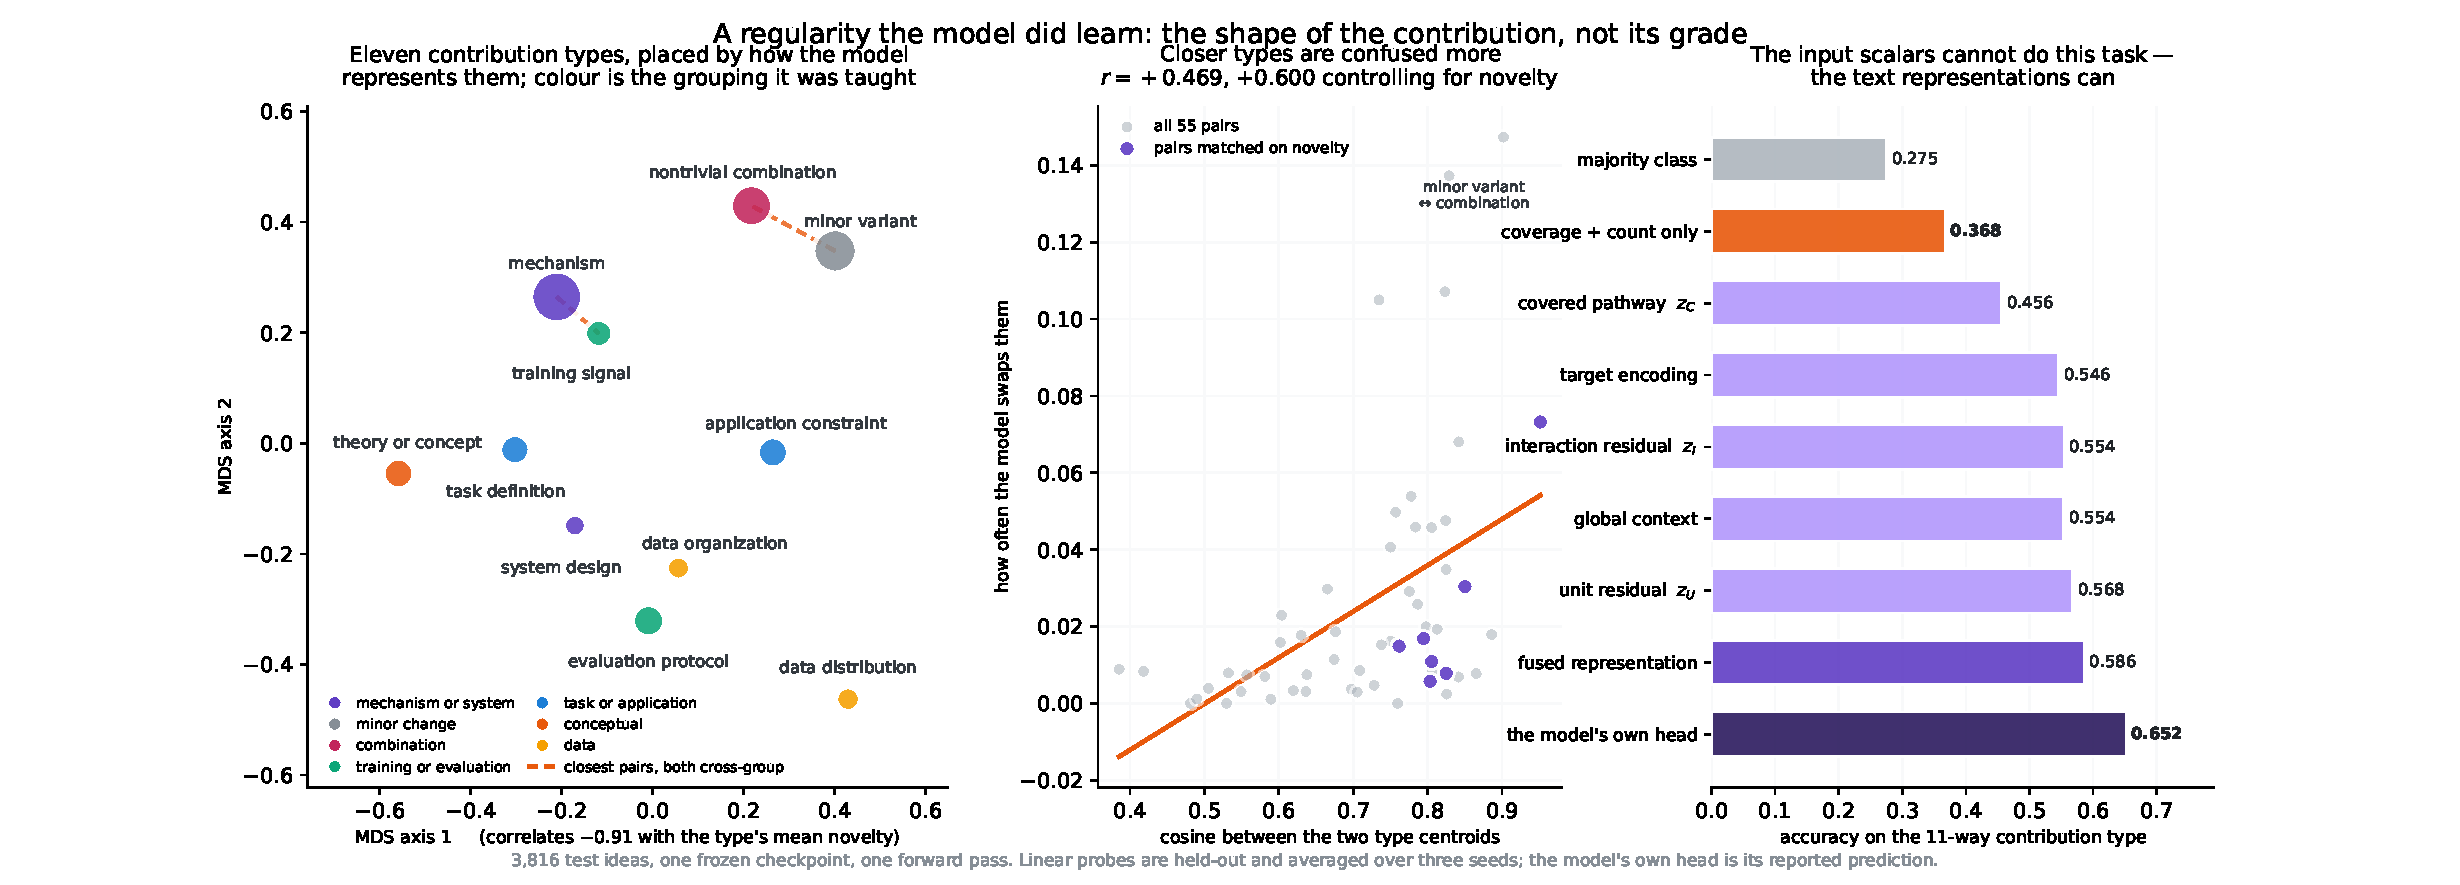
\includegraphics[width=\textwidth]{pic/contribution_map.pdf}
\caption{Left: the eleven contribution types, placed by classical multidimensional scaling
on the cosine distances between their centroids in the fused representation; two
dimensions carry $61.9\%$ of the centroid spread, and point area is class frequency.
Colour is the seven-way coarse grouping the model is \emph{supervised} with, so
same-coloured points sitting apart means the layout is not a replay of that supervision;
the dashed segments mark the two closest pairs in the whole map, both of which cross
groups. Centre: each of the 55 type pairs, its centroid cosine against how often the model
swaps the two. Right: held-out Accuracy of a linear probe for the eleven-way type,
averaged over three seeds.}
\label{fig:contribution-map}
\end{figure}

\paragraph{The types are laid out, and the layout predicts the model's own errors.}
Projecting the eleven centroids to two dimensions recovers $61.9\%$ of their spread, so the
arrangement is close to planar. Its first axis correlates at $-0.905$ with the mean novelty
grade of each type across the eleven classes, which places the conceptual and
task-defining contributions at one end and minor variants and recombinations at the other.

The arrangement is not decoration: it predicts where the model goes wrong. Over the 55
type pairs, the cosine between two centroids correlates at $r=0.469$ with how often the
model swaps those two types. The model never mistakes a new data distribution for a new
theoretical concept, the most distant pair in the map, and its single most frequent
confusion, minor variant against non-trivial combination, is one of its closest.

That correlation could be a restatement of the novelty axis, since types of similar
novelty would be confusable for that reason alone. It is not. Partialling out the
difference in mean novelty between the two types raises the correlation to $0.600$ rather
than removing it. The clearest case is \textsc{new\_mechanism} against
\textsc{new\_training\_signal}, whose mean grades differ by $0.05$ and which novelty
therefore cannot separate at all: they are the closest pair in the entire map at cosine
$0.951$, and among the novelty-matched pairs they are also the most often confused.

\paragraph{The layout disagrees with the grouping the model was taught.}
Training supervises a seven-way coarse grouping alongside the fine label, so the layout
could be that grouping made visible. It is not. Pairs inside a coarse group sit at mean
cosine $0.783$ and pairs across groups at $0.709$, a separation far smaller than the
spread within either set, and the four closest pairs in the map all cross groups. The
model places \textsc{minor\_variant} beside \textsc{nontrivial\_combination} at $0.902$
although the supervision assigns them to different coarse types, and it pulls
\textsc{new\_mechanism} away from \textsc{new\_system\_design} to $0.798$ although the
supervision groups them together. Both departures read as the more natural organisation:
a minor variant and a recombination are two degrees of reusing what exists, whereas a new
mechanism and a new system design are different kinds of contribution. We report this as
an observation about the representation, not as evidence that the taxonomy should be
redrawn; with only four same-group pairs available the comparison of the two means is
descriptive.

\paragraph{Where the knowledge sits.}
Probing each stage separately for the eleven-way type puts the covered pathway lowest at
$0.456$, the target encoding at $0.546$, the interaction residual at $0.554$, the global
context at $0.554$, the unit residual highest among the single pathways at $0.568$, and
the fused vector at $0.586$. Two readings follow. Every text-derived representation is
well clear of the $0.368$ the input scalars reach, so the contribution type is genuinely
carried by the encoded text rather than by the retrieval statistics. And the target
encoding alone already reaches $0.546$, which says that much of the type is legible from
how the idea is phrased --- a target that says it combines two things announces its own
category --- so the evidence pathways add less here than the gap to the model's $0.651$
head might suggest.
